\chapter{Entwurfsmuster}
Entwurfsmuster dienen in der Softwareentwicklung als Lösungsansätze für wiederkehrende Probleme.
Es handelt sich dabei nicht um fertigen Code, sondern vielmehr um konzeptionelle Bausteine, die zum Beispiel die Kommunikation unter Entwicklern unterstützen können.
Auch in diesem Programmentwurf finden sich Entwurfsmuster wieder.
Im Folgenden wird eines dieser Entwurfsmuster genauer erläutert.

\section{Beobachter}
Der Beobachter gehört zur Kategorie der Verhaltensmuster.
Kern des Konzeptes ist es, Änderungen an einem Ausgangsobjekt einer Anzahl anderer Objekte mitzuteilen.
Im Gegensatz zum Polling (ein Objekt fragt periodisch ab, ob sich der Zustand eines anderen geändert hat) findet hier Kommunikation nur im Änderungsfall statt.

Kernelement des Entwurfsmusters sind Subjekte, die von den Beobachtern observiert werden.
Ein Subjekt hat dabei die Möglichkeit, Beobachter an- und abzumelden, sowie diese zu benachrichtigen, wenn eine Veränderung vorliegt.
Bei dieser Benachrichtigung wird über alle registrierten Beobachter iteriert und deren Methode zur Aktualisierung aufgerufen.
Je nach Implementierung des Entwurfsmusters kann hier auch eine Payload mitgegeben werden.
Eine Darstellung des allgemeinen Schemas ist in \autoref{fig:beobachter-muster} zu sehen.

\begin{figure}
    \centering
    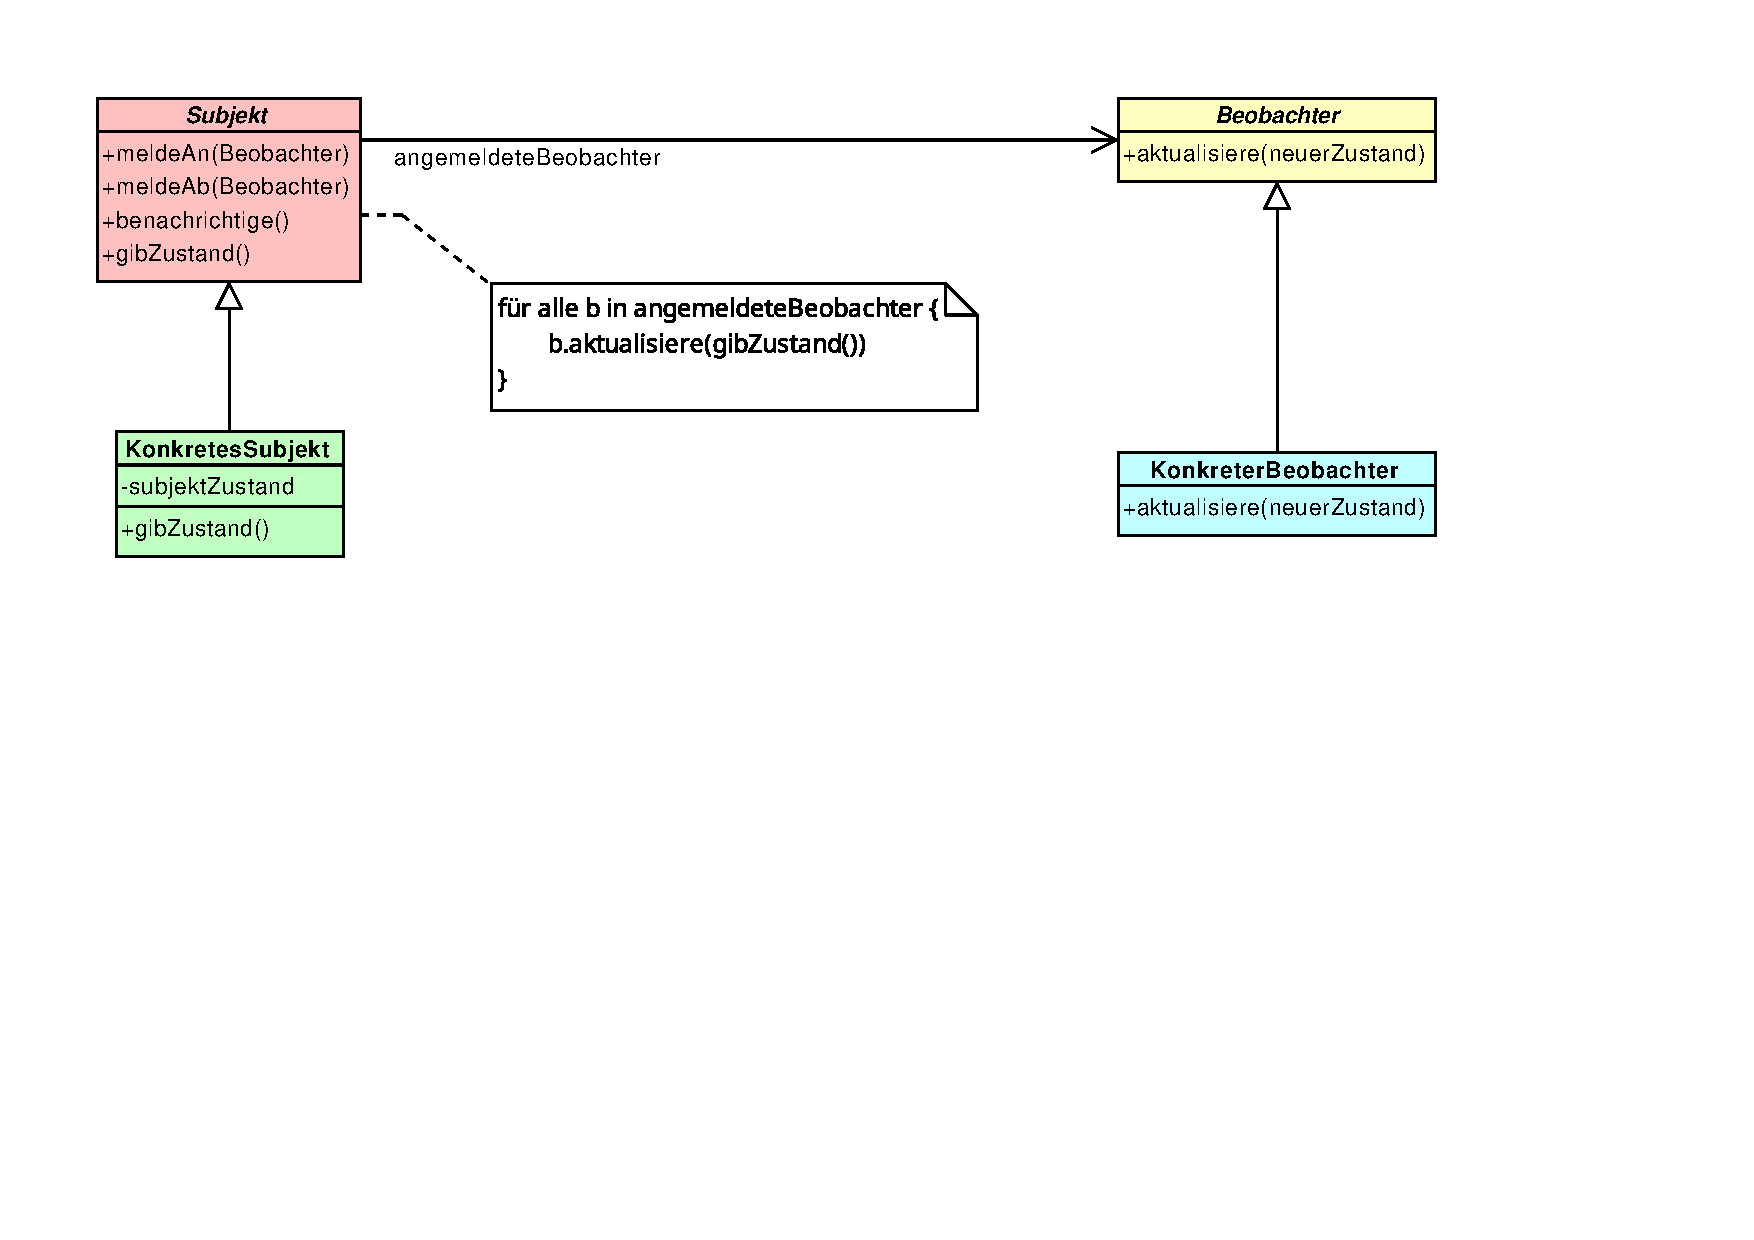
\includegraphics[width=\textwidth, trim = 0cm 10cm 3.5cm 0cm]{../VPP/Beobachter-Muster.pdf}
    \caption{Abstraktes UML-Diagramm des Beobachter-Entwurfsmusters}
    \label{fig:beobachter-muster}
\end{figure}

\subsection{Umsetzung im Programmentwurf}
In der grafischen Benutzeroberfläche des Fahrtkostenrechners spielen Knöpfe (JButtons) eine wichtige Rolle.
Knöpfe werden dabei ohne eigene Funktionalität instanziiert.
Stattdessen können für einen Knopf sogenannte \emph{ActionListener} registriert werden.
Dieser Vorgang (in \autoref{fig:beobachter-umsetzung} dargestellt) entspricht dem Beobachter-Entwurfsmuster.
Es wurde farblich hervorgehoben, welche Klassen der Umsetzung welcher Rolle des allgemeinen Schemas entsprechen.
\code{AbstractButton} entspricht dem abstrakten \code{Subjekt}, \code{ActionListener} dem abstrakten \code{Beobachter}, wobei hier für den abstrakten Beobachter ein Interface herangezogen wird anstelle einer Klasse.
Dieses Interface wird dann von der Klasse \code{FahrperiodenAbschliessService} implementiert.
\code{JButton} stellt die Implementierung des konkreten Subjekts (\code{KonkretesSubjekt}) dar.

\paragraph{Anmerkung}
\autoref{fig:beobachter-umsetzung} ist eine vereinfachte Darstellung der Implementierung des Java-Standards.
Insbesondere bei der Darstellung der \code{listenerList} wurde die Komplexität auf das Wesentliche heruntergebrochen, da die eigentliche Detailtiefe der Implementierung für die reine Demonstration des Entwurfsmusters hinderlich ist.

Die Verwendung des Entwurfsmusters ist \href{https://github.com/yschiebelhut/carpool-java/blob/fcc3bbaff5e8908a5f768b7fd3e79f1d2285acb6/0-carpool-java-plugin-ui/src/main/java/gui/FahrperiodeGUI.java#L103}{hier (Instanziierung des JButtons / Registrierung des ActionListeners)} und \href{https://github.com/yschiebelhut/carpool-java/blob/fcc3bbaff5e8908a5f768b7fd3e79f1d2285acb6/2-carpool-java-application/src/main/java/services/FahrperiodenAbschliessService.java}{hier (Implementierung des ActionListeners)} zu finden.
Die Implementierung der Subjekte ist Teil des Java-Standards.

\begin{figure}
    \centering
    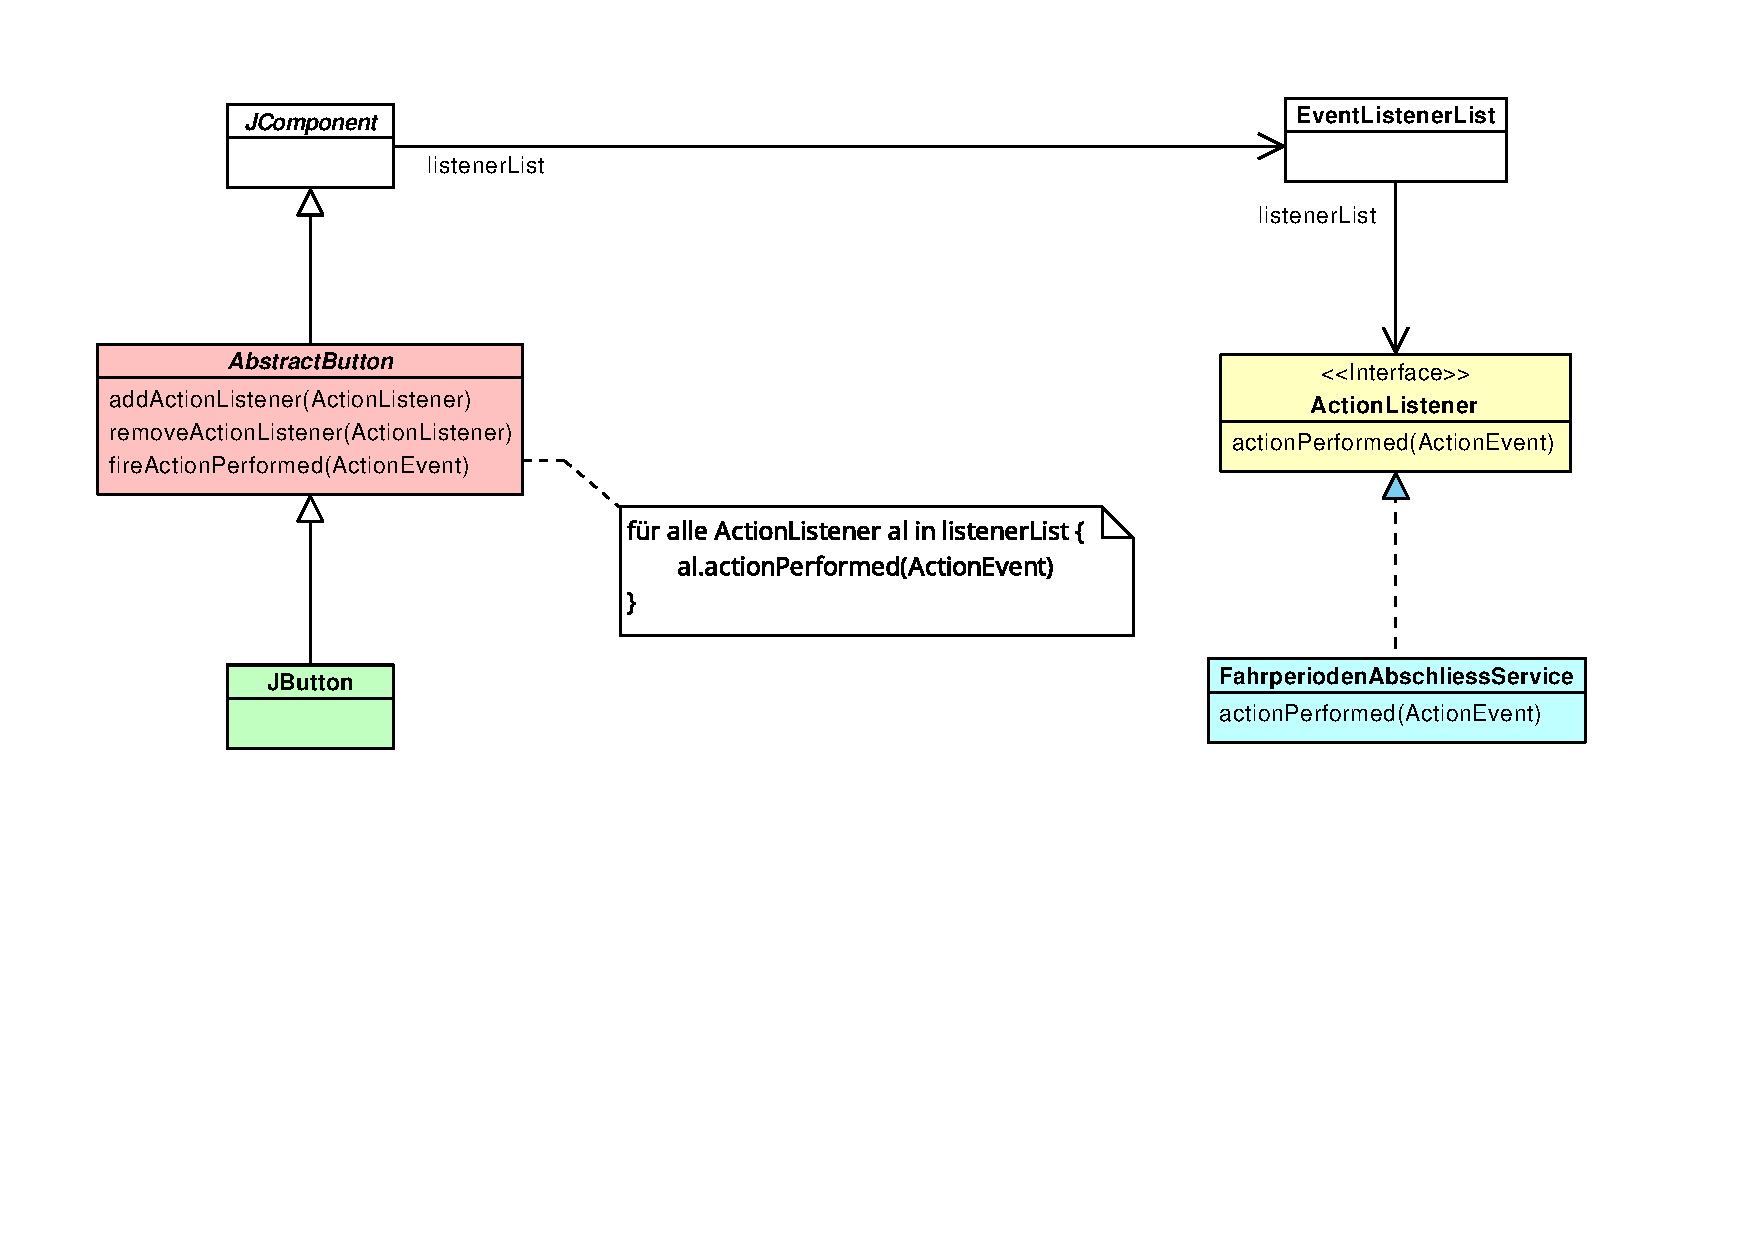
\includegraphics[width=\textwidth, trim = 0cm 7cm 0cm 0cm]{../VPP/Beobachter-Umsetzung.pdf}
    \caption{Konkrete Anwendung des Beobachter-Entwurfsmusters}
    \label{fig:beobachter-umsetzung}
\end{figure}